% Generated LaTeX file for compound CID: 81313
\documentclass[tikz]{standalone}
\definecolor{274A4A}{HTML}{274A4A}
\definecolor{FF0000}{HTML}{FF0000}
\begin{document}
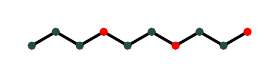
\begin{tikzpicture}[x=1pt,y=1pt]
  \draw[line width=1pt] (45.98,2.50) -- (54.64,-2.50);
  \draw[line width=1pt] (45.98,2.50) -- (37.32,-2.50);
  \draw[line width=1pt] (71.96,-2.50) -- (63.30,2.50);
  \draw[line width=1pt] (71.96,-2.50) -- (80.62,2.50);
  \draw[line width=1pt] (97.94,2.50) -- (89.28,-2.50);
  \draw[line width=1pt] (54.64,-2.50) -- (63.30,2.50);
  \draw[line width=1pt] (37.32,-2.50) -- (28.66,2.50);
  \draw[line width=1pt] (28.66,2.50) -- (20.00,-2.50);
  \draw[line width=1pt] (80.62,2.50) -- (89.28,-2.50);
  \filldraw[fill=FF0000, draw=none] (45.98,2.50) circle (1.5pt);
  \filldraw[fill=FF0000, draw=none] (71.96,-2.50) circle (1.5pt);
  \filldraw[fill=FF0000, draw=none] (97.94,2.50) circle (1.5pt);
  \filldraw[fill=274A4A, draw=none] (54.64,-2.50) circle (1.5pt);
  \filldraw[fill=274A4A, draw=none] (37.32,-2.50) circle (1.5pt);
  \filldraw[fill=274A4A, draw=none] (63.30,2.50) circle (1.5pt);
  \filldraw[fill=274A4A, draw=none] (28.66,2.50) circle (1.5pt);
  \filldraw[fill=274A4A, draw=none] (80.62,2.50) circle (1.5pt);
  \filldraw[fill=274A4A, draw=none] (20.00,-2.50) circle (1.5pt);
  \filldraw[fill=274A4A, draw=none] (89.28,-2.50) circle (1.5pt);
\end{tikzpicture}
\end{document}